\documentclass[10pt]{beamer}

\usetheme{default}

\usepackage[utf8]{inputenc}
\usepackage[russian]{babel}
\usepackage[OT1]{fontenc}
\usepackage{amsmath}
\usepackage{amsfonts}
\usepackage{amssymb}
\usepackage{graphicx}
\usepackage{etoolbox}
\usepackage{caption}
\usepackage{subcaption}
\usepackage{pifont}
\usepackage{xcolor}
\usepackage{framed}
\definecolor{shadecolor}{cmyk}{0,0,0,1}
\usepackage{listings}

\lstset{
    backgroundcolor=\color{lightgray},
    commentstyle=\color{blue},
    frame=single
    breakatwhitespace, 
    language=python, 
    columns=fullflexible, 
    keepspaces, 
    breaklines, 
    tabsize=3, 
    subfigurehowstringspaces=false, 
    extendedchars=true,
    numbers=left
}

\makeatletter

\DeclareMathOperator*{\argmin}{arg\,min}

\setbeamercolor{title}{fg=white}
\setbeamercolor{frametitle}{fg=black}
\setbeamerfont*{title}{family=\sffamily,size=\LARGE}

\setbeamerfont{page number in head/foot}{size=\scriptsize}
\setbeamertemplate{footline}[frame number]
\let\otp\titlepage
\renewcommand{\titlepage}{\otp\addtocounter{framenumber}{-1}}

\setbeamertemplate{background canvas}{%
	\ifnumequal{\c@framenumber}{0}{%
      
\includegraphics[width=\paperwidth,height=\paperheight]{images/cover.png}
   }{%
      \ifnumequal{\c@framenumber}{\inserttotalframenumber}{
         
\includegraphics[width=\paperwidth,height=\paperheight]{images/back.png}
      }{%
         % Other frames
      }%
   }%
}

\makeatother

\beamertemplatenavigationsymbolsempty

\author{Владимир Гулин}
\title{\newline \newline \newline Лекция 10 \\ Алгоритмические композиции\\
Кульминация и развязка}

\begin{document}

\begin{frame}[plain]
\titlepage
\end{frame}

\begin{frame}{План лекции}
\tableofcontents
\end{frame}

% =======================
\section{Напоминание}
% =======================

\begin{frame}{Задача обучения с учителем}
\begin{block}{Постановка задачи}
\end{block}

Пусть дан набор объектов $\mathcal{D} = \{(\mathbf{x}_i, y_i)\},
\; \mathbf{x}_i \in \mathcal{X},
\; y_i \in \mathcal{Y},
\; i \in 1, \ldots, N$, полученный из неизвестной закономерности $y =
f(\mathbf{x})$. Необходимо построить такую $h(\mathbf{x})$, которая наиболее точно
аппроксимирует $f(\mathbf{x})$.

\vspace{1em}
Будем искать неизвестную 
\[
    h(\mathbf{x}) = C(a_1(\mathbf{x}), \ldots, a_T(\mathbf{x}))
\]

$a_i(\mathbf{x}):\mathcal{X} \rightarrow \mathcal{R}, \,\, \forall i \in
\{1,\ldots, T\}$ - базовые модели 

$C: \mathcal{R} \rightarrow \mathcal{Y}$ - решающее правило
\end{frame}


\begin{frame}{Алгоритмические композиции}
\begin{block}{Simple Voting}
\end{block}
\[
    h(\mathbf{x}) = \frac{1}{T} \sum \limits_{i=1}^{T} a_i(\mathbf{x})
\]
\begin{block}{Weighted Voting}
\end{block}
\[
    h(\mathbf{x}) = \frac{1}{T} \sum \limits_{i=1}^{T}b_i a_i(\mathbf{x}), \,\,
    b_i \in \mathcal{R}
\]
\begin{block}{Mixture of Experts}
\end{block}
\[
    h(\mathbf{x}) = \frac{1}{T} \sum \limits_{i=1}^{T}b_i(\mathbf{x}) a_i(\mathbf{x}), \,\,
    b_i(\mathbf{x}): \mathcal{X} \rightarrow \mathcal{R}
\]
\end{frame}

% =======================
\section{Бустинг}
% =======================

\begin{frame}{Идея бустинга}
\begin{block}{Снова выбираем ноутбук}
\end{block}
    Вместо того, чтобы спрашивать у всех экспертов, какой ноутбук выбрать,
    будем после каждого очередного мнения менять наш вопрос.
    
\vspace{1em}
\begin{itemize}
    \item Более реалистичная модель
    \item Уточняем наш вопрос в зависимости от ответов предыдущих экспертов
\end{itemize}
\end{frame}

\begin{frame}{Boosting vs Bagging}
\begin{columns}[C]
    \begin{column}{.5\textwidth}
        \begin{block}{Стрельба в тире}
        \end{block}
        \begin{center}
            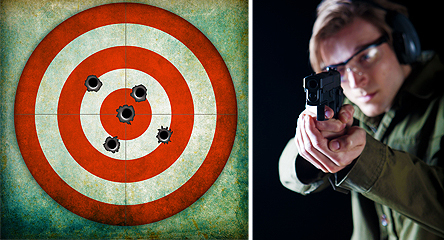
\includegraphics[scale=0.33]{images/tir.jpg}
        \end{center}
    \end{column}
    \begin{column}{.5\textwidth}
        \begin{block}{Игра в гольф}
        \end{block}
        \begin{center}
            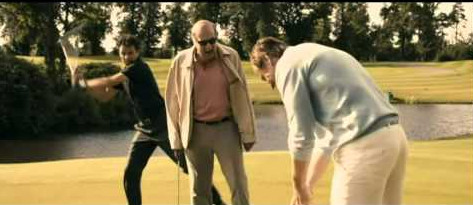
\includegraphics[scale=0.35]{images/golf.jpg}
        \end{center}
    \end{column}
\end{columns}
\end{frame}

\begin{frame}{Бустинг для задачи бинарной классификации}
Пусть
\[
    Y={-1, +1}, \quad a_i : X \rightarrow \{ -1, 0, +1 \}, \,\, i=1 \ldots T
\]

\vspace{1em}
Будем строить модель взвешенного голосования:
\[
    h(\mathbf{x}) = sign \left( \sum \limits_{i=1}^{T} b_i a_i(\mathbf{x})
    \right), \, b_i \in \mathcal{R}
\]

\vspace{1em}
Функция потерь
\[
    err(h) = \frac{1}{N} \sum \limits _{j=1}^N I(y_j \neq h(\mathbf{x}_j))
\]
\end{frame}

\begin{frame}{Ключевые идеи бустинга}
\begin{itemize}
\item Используем ``слабые'' модели $a_i$
\item Последовательно применяем слабые модели к ``слегка'' изменяемым версиям
    оригинальных данных
\item При добавлении очередной модели $a_i$, предыдущие $i-1$ моделей не
    меняются
\item Аппроксимируем функцию потерь гладкой функцией
\end{itemize}
\end{frame}

\begin{frame}{Аппроксимация пороговой функции экспонентой}
Очевидно, что верно соотношение
\[
    I(y \neq a(\mathbf{x})) = I(y \cdot a(\mathbf{x}) \le 0) \le e^{-y \cdot a(\mathbf{x})}
\]
Тогда ошибку композиции $h(\mathbf{x})$ можно оценить сверху
\[
    0 \le err(h) = \frac{1}{N} \sum \limits _{j=1}^N I(y_j \neq h(\mathbf{x}_j)) \le
\]
\[
    \le \frac{1}{N} \sum \limits _{j=1}^N exp \left(-y_j \sum \limits _{i=1}^{T-1} b_i
    a_i(\mathbf{x}) \right) \cdot exp(-y_j b_T a_T( \mathbf{x} )) \rightarrow 0
\]
\end{frame}

\begin{frame}{AdaBoost(Freund \& Shapire 1995)}
\begin{enumerate}
    \item Инициализировать веса объектов $w_j=1/N, \, j=1,2,\ldots,N$.
    \item Для всех $i$ от $1$ до $T$:
    \begin{enumerate}[(a)]
        \item Построить классификатор $a_i(\mathbf{x})$, используя веса $w_j$
        \item Вычислить
        \[
            err_i = \frac{\sum_{j=1}^N w_j I(y_j \neq a_i(\mathbf{x}_j)
            )}{\sum_{j=1}^N w_j}
        \]
        \item Вычислить 
        \[
            b_i = \log{\frac{1-err_i}{err_i}}
        \]
        \item Присвоить $w_j \rightarrow w_j \cdot exp[b_i \cdot I(y_j \neq
            a_i(\mathbf{x}_j))], \, j=1,\ldots,N.$
\end{enumerate}
    \item $h(\mathbf{x}) = sign\left[ \sum _{i=1}^T b_i a_i(\mathbf{x})   \right ]$
\end{enumerate}
\end{frame}

\begin{frame}{AdaBoost. Пример}
    \begin{center}
        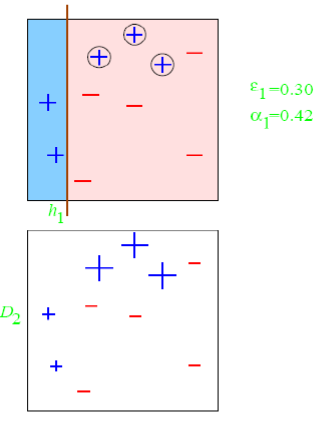
\includegraphics[scale=0.3]{images/adaboost.png}
    \end{center}
\end{frame}

\begin{frame}{AdaBoost. Пример}
    \begin{center}
        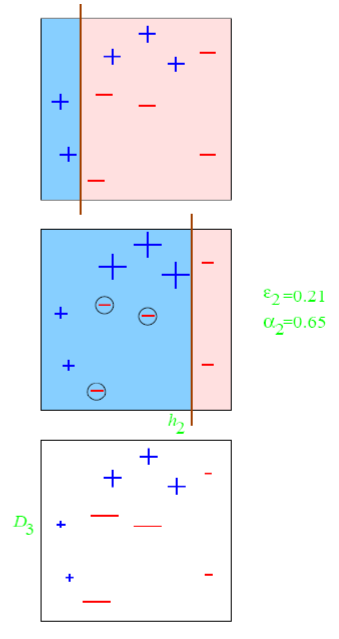
\includegraphics[scale=0.3]{images/adaboost2.png}
    \end{center}
\end{frame}

\begin{frame}{AdaBoost. Пример}
    \begin{center}
        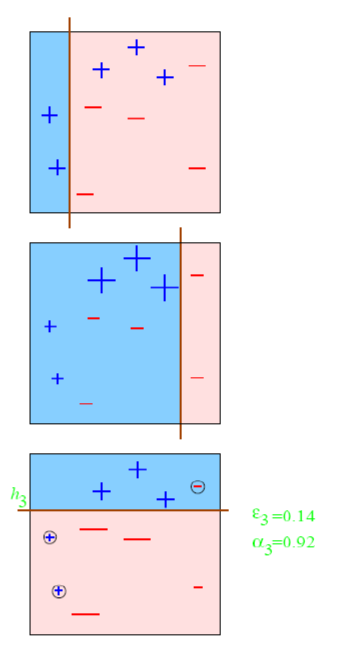
\includegraphics[scale=0.3]{images/adaboost3.png}
    \end{center}
\end{frame}

\begin{frame}{AdaBoost. Пример}
    \begin{center}
        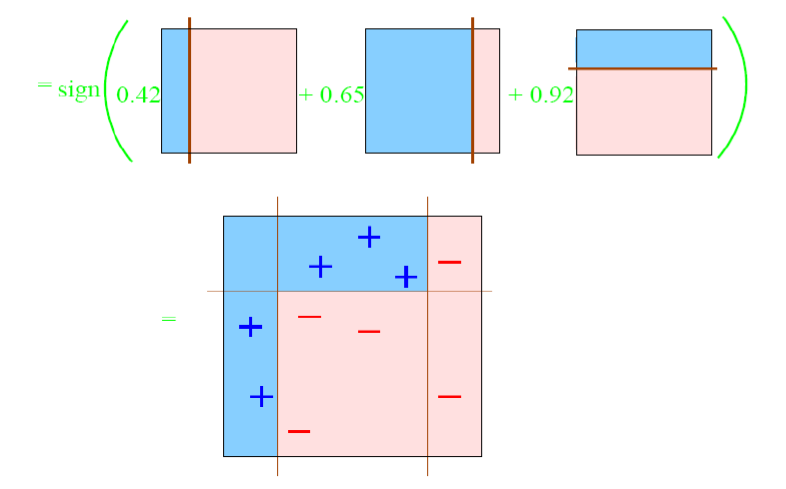
\includegraphics[scale=0.3]{images/adaboost4.png}
    \end{center}
\end{frame}

\begin{frame}{Почему именно аппроксимация экспонентой?}
\begin{center}
    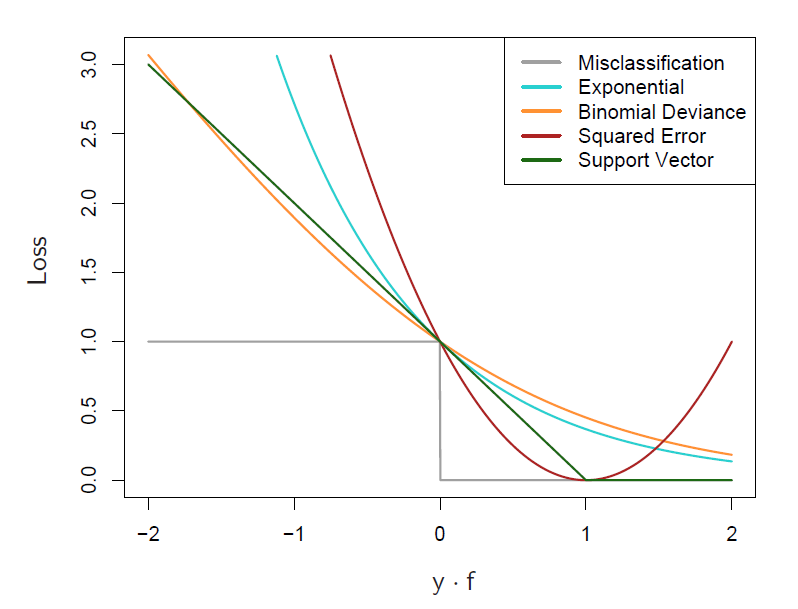
\includegraphics[scale=0.3]{images/exploss.png}
\end{center}
\end{frame}

\begin{frame}{Какие базовые модели выбрать?}
\begin{block}{Теорема:}
\end{block}
Если на каждой итерации метод обучения позволяет построить базовую модель,
такую что число верных классификаций больше, чем число неверных. Тогда метод
обучения сходится за конечное число шагов.

\vspace{1em}
\begin{itemize}
    \item Базовые модели должны обладать достаточной сложностью, чтобы
        обеспечить это требование.
\end{itemize}

\vspace{1em}
\begin{block}{Вопрос:}
\end{block}
\begin{itemize}
    \item Можно ли использовать в качестве базовых моделей линейную регрессию
        для алгоритма AdaBoost?
\end{itemize}
\end{frame}

\begin{frame}{Boosting decision stumps}
\begin{center}
    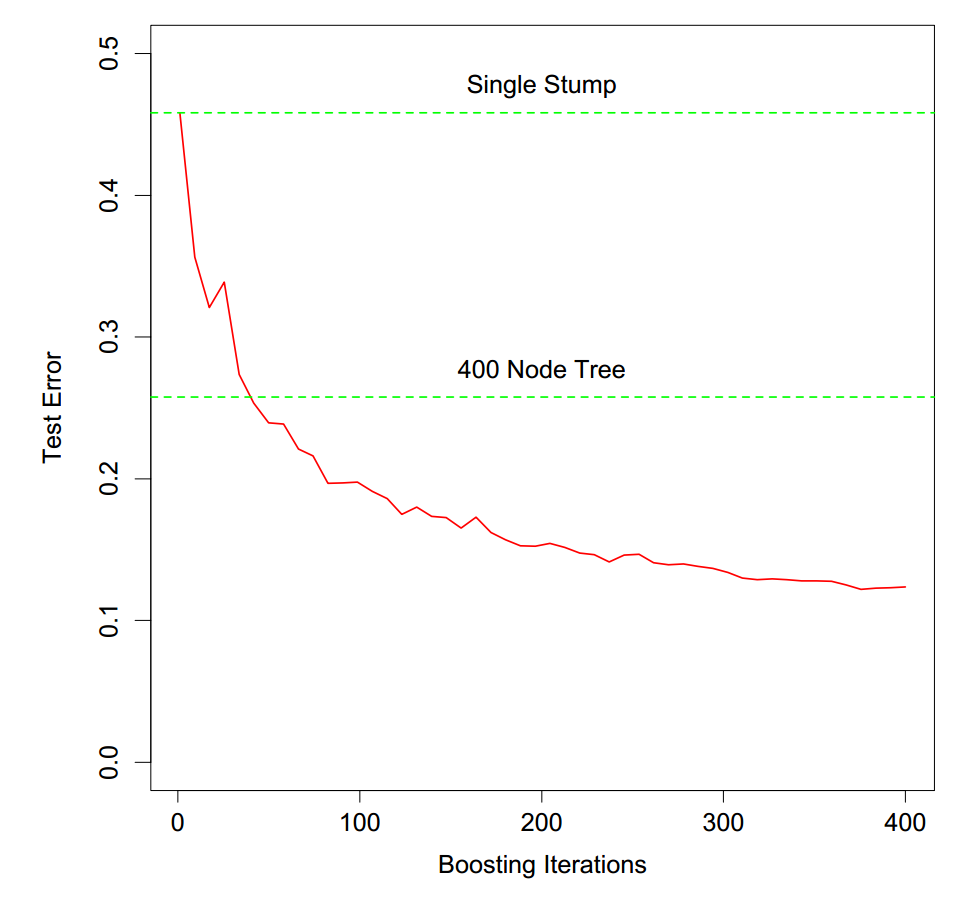
\includegraphics[scale=0.25]{images/boostingstumps.png}
\end{center}
\end{frame}

\begin{frame}{Удивительные факты о бустинге}
\begin{center}
    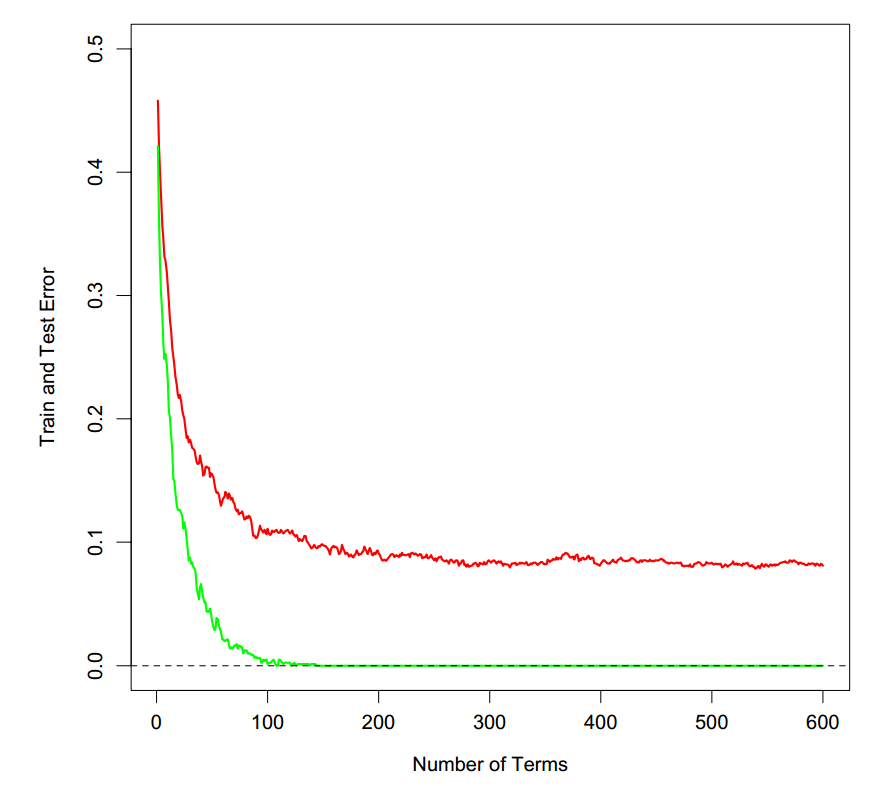
\includegraphics[scale=0.2]{images/interestingboosting.png}
\end{center}
\begin{itemize}
    \item не переобучается с увеличением числа итераций
\end{itemize}
\end{frame}

\begin{frame}{Bias \& variance}
Оценка ожидания ошибки на некоторой точки $\mathbf{x}_0$
\[
    Err(\mathbf{x}_0) = Bias^2 + Variance + Noise (Irreducible\,\, Error)
\]
\begin{itemize}
    \item Бэггинг уменьшает $Variance$
    \item Бустинг уменьшает и $Variance$ и $Bias$. Причем начальные модели отвечают
    за уменьшение именно $Bias$, а остальные за уменьшение $Variance$.
\end{itemize}
\end{frame}

\begin{frame}{Применение AdaBoost}
\begin{block}{Viola–Jones object detection framework}
\end{block}
\begin{columns}[C]
    \begin{column}{.5\textwidth}
    \begin{center}
        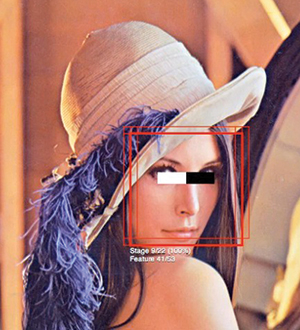
\includegraphics[scale=0.3]{images/violalena.jpg}
    \end{center}
    \end{column}
    \begin{column}{.5\textwidth}
        \begin{center}
            
\includegraphics[scale=0.3]{images/violabase.jpg}
        \end{center}
    \end{column}
\end{columns}
\[
    a_i(\mathbf{x}_j) = \left[ \begin{array}{c} \alpha_{i} \quad \text{если}
            \,\, 
            f_i(\mathbf{x}_j) > \theta_i \\ 
            \beta_i \quad \text{иначе}
                               \end{array} \right. 
\]
\end{frame}

\begin{frame}{AdaBoost. Итоги}
\begin{itemize}
    \item[\color{green}\ding{52}] Алгоритм прост
    \item[\color{green}\ding{52}] Накладные расходы бустинга минимальны. Время
    построения определяется временем построения базовых моделей
    \item[\color{green}\ding{52}] Показывает хорошую обобщающую способность
    \item[\color{green}\ding{52}] Имеет возможность идентификации шумовых объектов
    \item[\color{red}\ding{54}] Жадное добавление алгоритмов приводит к
    неоптимальности композиции
    \item[\color{red}\ding{54}] Склонен к переобучению при наличии шума в данных
    (опять же из-за экспоненциальной функции потерь)
    \item[\color{red}\ding{54}] Переобучается при ``малом'' количестве данных
\end{itemize}


\end{frame}

% =======================
\section{Градиентный бустинг}
% =======================

\begin{frame}{Градиентный бустинг}
Модель взвешенного голосования
\[
    h(\mathbf{x}) = \sum \limits _{i=1}^T b_i a_i(\mathbf{x}), \quad \mathbf{x}
    \in X, b_i \in R
\]

\vspace{1em}
Ошибка композиции на обучающей выборке
\[
    err(h) = \sum \limits _{j=1}^N L(y_j, \sum \limits _{i=1}^{T-1} b_i
    a_i(\mathbf{x}_j)  + b \cdot a(\mathbf{x}_j)) \rightarrow \min \limits_{b,a}
\]

\vspace{1em}
\begin{itemize}
    \item Применяем жадную стратегию добавления моделей
    \item Как и раньше оставляем построенные алгоритмы с весами неизменными
\end{itemize}
\end{frame}

\begin{frame}{Градиентный бустинг}
Применим метод минимизации (метод наискорейшего спуска) $err(h)$:

\vspace{1em}
Тогда
\[
    h_{i,j} = h_{i-1, j} - \eta \cdot err'(h_{i-1, j}), \quad j=1,\ldots,N
\]
$\eta$ - шаг спуска

\vspace{1em}
\begin{block}{Основная идея:}
\end{block}
На каждом шаге алгоритма будем искать модель $a_i$, которая аппроксимировала бы
вектор антиградиента.
\end{frame}

\begin{frame}{Gradient boosting algorithm}
\begin{enumerate}
    \item Инициализировать $h_0(\mathbf{x}) = argmin_{\gamma} \sum \limits_{j=1}^{N} L(y_j, \gamma)$
    \item Для всех $i$ от $1$ до $T$:
        \begin{enumerate}[(a)]
            \item Для всех $j=1,2,\ldots,N$ вычислить
                \[
                    g_{i,j} = - \left[ \frac{\partial L(y_j, h(\mathbf{x}_j))}{\partial
                    h(\mathbf{x}_j)}  \right]_{h=h_{i-1}}
                \]
            \item Построить базовую модель $a_i$ на ответах $g_{i,j}$
                \[
                    a_i = \argmin \limits _{\beta, a} \sum \limits _{j=1}^{N} (g_{i,j} -
                    \beta a(\mathbf{x}_j))^2
                \]
            \item Определить вес $b_i$
                \[
                    b_i = \argmin \limits _b  \sum \limits _{j=1}^N L(y_j,
                    h_{i-1}(\mathbf{x}) + b \cdot a_i(\mathbf{x}_j))
                \]
            \item Присвоить $h_{i}(\mathbf{x}) = h_{i-1}(\mathbf{x}) + b_i \cdot  a_i(\mathbf{x})$
        \end{enumerate}
    \item Вернуть $h(\mathbf{x}) = h_{T}(\mathbf{x})$
\end{enumerate}
\end{frame}

\begin{frame}{Gradient boosting \& overfitting}
\begin{center}
    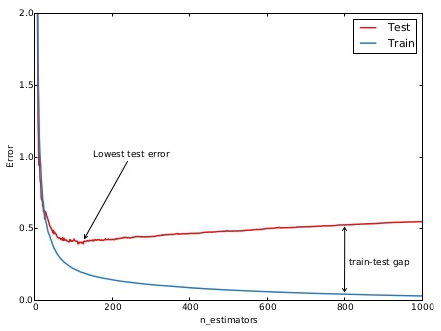
\includegraphics[scale=0.4]{images/gbtover.png}
\end{center}
\begin{itemize}
    \item Необходимо подбирать число деревьев на валидационной выборке
\end{itemize}
\end{frame}

\begin{frame}{Shrinkage}
\begin{block}{Идея:}
\end{block}
\begin{itemize}
    \item Будем делать шаг каждым алгоритмом с некоторым дисконтом
\end{itemize}
\begin{columns}[C]
    \begin{column}{.5\textwidth}
        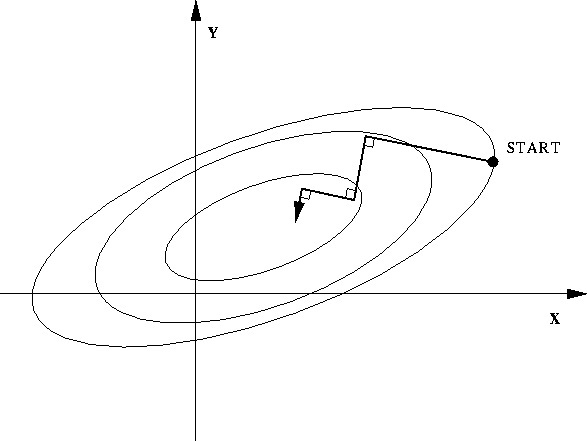
\includegraphics[scale=0.3]{images/stepestdecent.png}
    \end{column}
    \begin{column}{.5\textwidth}
        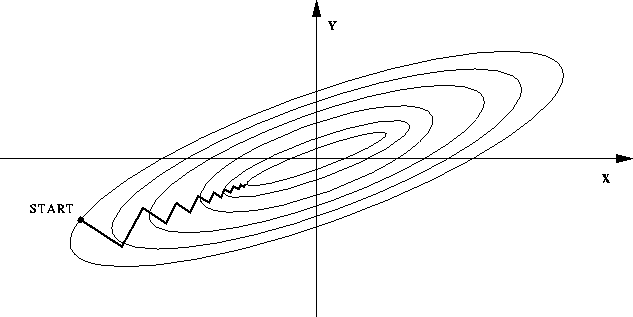
\includegraphics[scale=0.3]{images/shrinkage.png}
    \end{column}
\end{columns}
\[
    h_{i}(\mathbf{x}) = h_{i-1}(\mathbf{x}) + \mu \cdot b_i \cdot  a_i(\mathbf{x})
\]
\begin{itemize}
    \item Дадим гольфисту тяжелую клюшку, чтоб он не мог ударить сильно
\end{itemize}
\end{frame}

\begin{frame}{Stohastic gradient boosting}
\begin{center}
    Stohastic gradient boosting = Gradient Boosting + Bagging
\end{center}

\vspace{1em}
\begin{block}{Идея:}
\end{block}
\begin{itemize}
    \item Для построения очередного алгоритма используются случайная
        подвыборка, полученная алгоритмом выбора без возвращения
    \item Выдадим гольфисту шары разной формы
\end{itemize}

\vspace{1em}
\begin{block}{Преимущества}
\end{block}
\begin{itemize}
    \item Уменьшается время обучения
    \item Лучше сходится (эквивалентно методу стохастического градиентного
        спуска)
    \item Имеет более высокую обобщающую способность
\end{itemize}
\end{frame}

\begin{frame}{Shrinkage \& Subsampling}
\begin{center}
    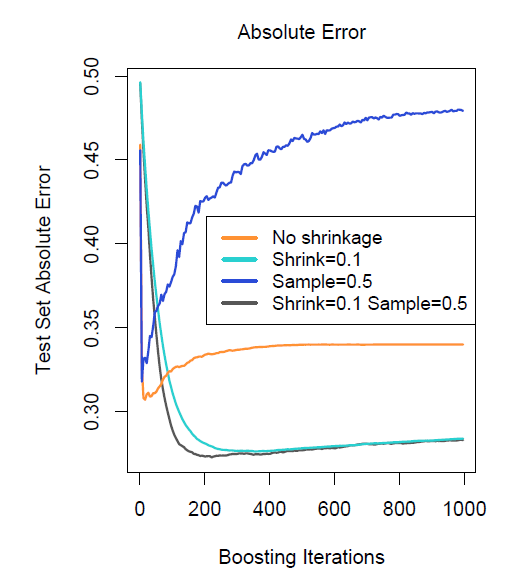
\includegraphics[scale=0.4]{images/shrsub.png}
\end{center}
\end{frame}

\begin{frame}{Regularization in leafs}
\begin{block}{Идея:}
\end{block}
\begin{itemize}
    \item Не все листы имеют одинаковый вклад
    \item ``Важность'' листа зависит от числа объектов в нем
    \item Дадим гольфисту палку вместо клюшки
\end{itemize}
\begin{center}
    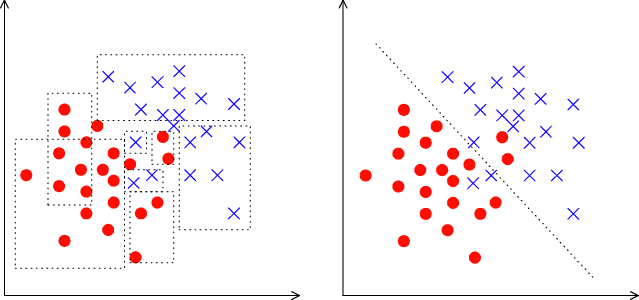
\includegraphics[scale=0.3]{images/leafs.png}
\end{center}
\begin{block}{Варианты решения:}
\end{block}
\begin{itemize}
    \item Ограничить минимальное число примеров в листьях
    \item Домножить значения в листьях на некоторую фукцию, зависящую от
        количества примеров
\end{itemize}
\end{frame}

\begin{frame}{OOB \& Feature Importance}
\begin{columns}[C]
    \begin{column}{.4\textwidth}
        \begin{center}
            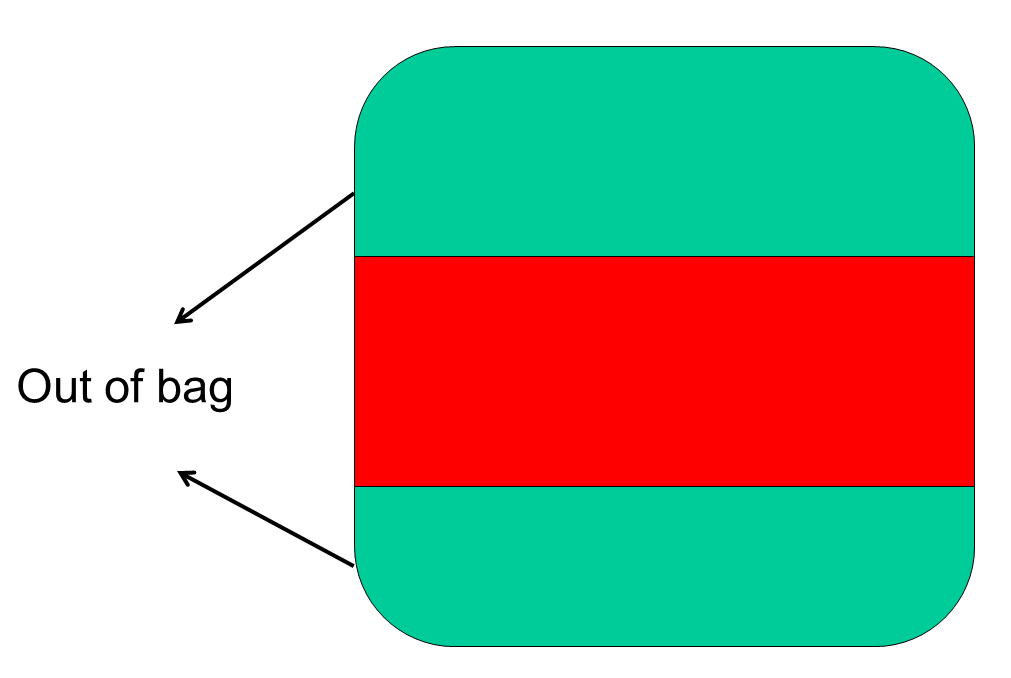
\includegraphics[scale=0.15]{images/outofbag.png}
        \end{center}
    \end{column}
    \begin{column}{.6\textwidth}
        \begin{center}
            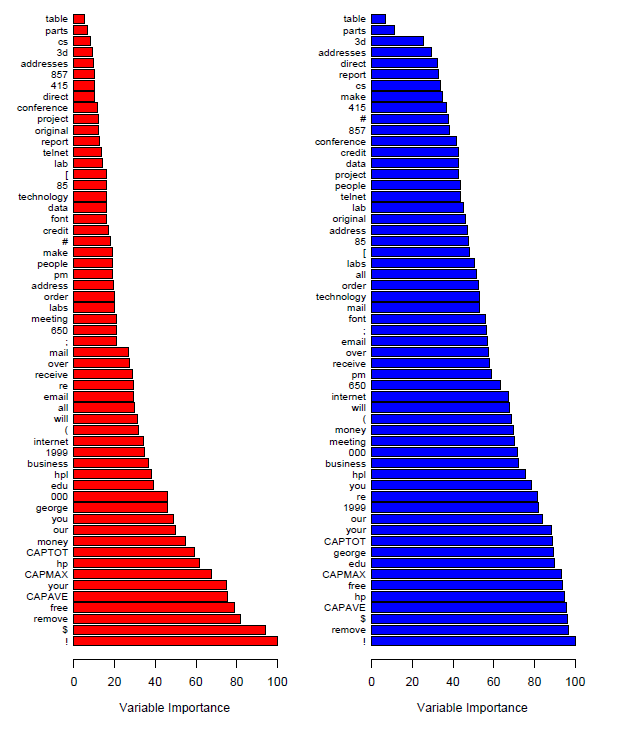
\includegraphics[scale=0.2]{images/impotance.png}
        \end{center}
    \end{column}
\end{columns}
\end{frame}

\begin{frame}{Gradient boosting algorithm complexity}
\begin{itemize}
    \item Вычисление градиента $O(g(N))$ 
    \item Построение модели (дерева) $O(ND)$
    \item Вычисление предсказания $O(N)$
\end{itemize}

\vspace{1em}
Построение дерева может быть эффективно распараллелено по фичам. Поэтому в
целом быстро.
\end{frame}

\begin{frame}{Gradient boosting. Итоги}
\begin{itemize}
    \item Gradient boosting - общий алгоритм бустинга. Позволяет работать с
        произвольными функциями потерь и пространствами ответов.
    \item Чаще всего применяется с деревьями решений.
    \item Показывает наилучшее качество для задач классификации, регресии и
        ранжирования.
    \item Применять надо с регуляризацией, иначе результаты могут получиться
        удручающими.
\end{itemize}
\begin{block}{Вопрос:}
\end{block}
\begin{itemize}
    \item А что делать если функция не дифференцируема?
\end{itemize}
\end{frame}

\begin{frame}{Стохастические алгоритмы и бустинг. Итоги}
\begin{itemize}
    \item[\color{green}\ding{52}] Бустинг лучше работает для больших обучающих
    выборок в ситуациях когда в данных имеются сложные зависимости.
    \item[\color{green}\ding{52}] Стохастические методы лучше работают для коротких
    обучающих выборок
    \item[\color{green}\ding{52}] Стохастические алгоритмы можно эффективно
    распараллелить. Бустинг предполагает последовательное построение
    композиции.
    \item[\color{green}\ding{52}] RSM наиболее эффективен в пространствах большой
    размерности
    \item[\color{green}\ding{52}] Для бустинга лучше строить длинные композиции из
    слабых моделей, чем короткие из сильных
\end{itemize}

\begin{block}{Вопрос:}
\end{block}
\begin{itemize}
    \item А всегда ли стоит использовать деревянные модели bagging \& boosting?
\end{itemize}
\end{frame}

% =======================
\section{Мета-алгоритмы}
% =======================

\begin{frame}{BagBoo \& BooBag}
\begin{block}{Идея:}
\end{block}
\begin{itemize}
    \item Объединим стратегии бустинга и бэггинга
\end{itemize}
\begin{center}
    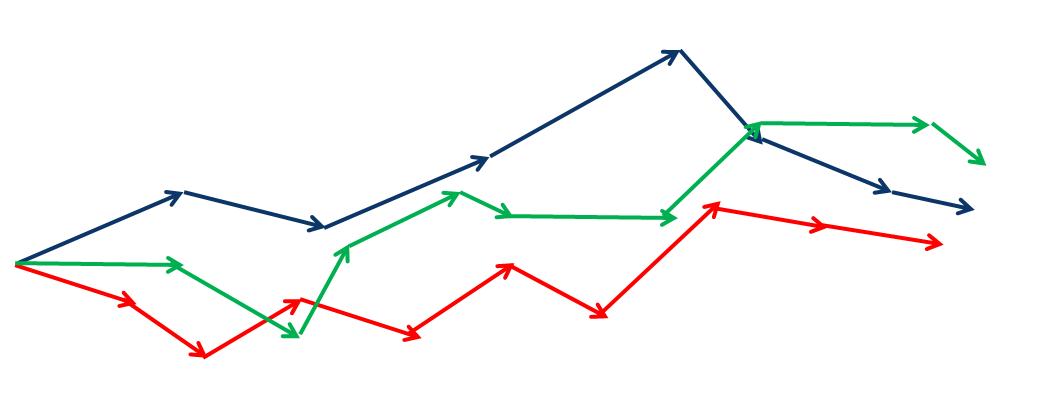
\includegraphics[scale=0.25]{images/bagboo.png}
\end{center}
\begin{itemize}
    \item Если объединять бустинг бэггингом то BagBoo
    \item Если объединять бэггинг бустингом то BooBag
\end{itemize}
\end{frame}

\begin{frame}{Итоги}
\begin{itemize}
    \item Бустингом бэггинг не испортишь! (и наоборот)
    \item При таком подходе реальное качество почти неограничено... все
        упирается в число деревьев
    \item К сожалению, не получается применять в больших высоконагруженных
        системах
    \item Если есть много машин, то можно оценить верхнюю границу качества
        системы машинного обучения
\end{itemize}
\end{frame}

\begin{frame}[fragile]{Задача}

{\bf Дано:} Имеется набор данных из системы поискового антиспама. \\
{\bf Требуется:} Требуется сравнить классификаторы, основанные на
алгоритмических композициях, с методом опорных векторов.

\vspace{1em}
Пошаговая инструкция
\begin{enumerate}
    \item Скачать данные и запустить шаблон кода на python
    \url{http://goo.gl/ASDF7U}
\begin{shaded}
{\color{green} \begin{verbatim}
$ python compos.py -h
$ python compos.py -tr spam.train.txt -te spam.test.txt
\end{verbatim}}
\end{shaded}
    \item Подобрать параметры 3х алгоритмических композиций, чтобы они превосходили
    по качеству SVM.
    \item Построить графики качества классификации, в зависимости от числа базовых
    моделей.
\end{enumerate}

\end{frame}

\begin{frame}[fragile]{Дз по алгоритмическим композициям:}
    \begin{block}{Задание:}
\end{block}
    Реализовать один из алгоритмов машинного обучения, являющегося композицией
    алгоритмов и применить свою реализацию на данных из репозитория UCI.

\vspace{1em}
Имеется 12 вариантов задания:\\
Для того, чтобы узнать свой вариант необходимо выполнить функцию:
\begin{shaded}
{ \color{green} \begin{verbatim}
    def ComputeMyTaskNumber(your_name):
        return 1 + hash(your_name) % 12
\end{verbatim}}
\end{shaded}
где your\_name - это ваши фамилия и имя латиницей (например 'Pupkin Vasiliy')
\end{frame}

\begin{frame}[fragile]{Варианты:}
\begin{enumerate}
    \item Реализация модельного дерева решений с линейной регрессией в листьях
    \item Реализация алгоритма Random Forest (базовый алгоритм CART)
    \item Реализация алгоритма AdaBoost (базовый алгоритм CART)
    \item Реализация алгоритма градиентного бустинга с квадратичной функцией
        потерь. В качестве базового алгоритма использовать алгоритм CART.
    \item Реализация алгоритма градиентного бустинга с логистической футкцией
        потерь. В качестве базового алгоритма использовать алгоритм CART.
    \item Реализация алгоритма градиентного бустинга с квадратичной функцией
        потерь. В качестве базового алгоритма использовать алгоритм CART с RSM.
\end{enumerate}
\end{frame}

\begin{frame}[fragile]{Варианты:}
\begin{enumerate}
    \setcounter{enumi}{6}
    \item Реализация алгоритма градиентного бустинга с логистической футкцией
        потерь. В качестве базового алгоритма использовать алгоритм CART c RSM.
    \item Реализация алгоритма стохастического градиентного бустинга с
        квадратичной функцией потерь. В качестве базового алгоритма
        использовать алгоритм CART.
    \item Реализация алгоритма стохастического градиентного бустинга с
        логистической футкцией потерь. В качестве базового алгоритма
        использовать алгоритм CART.
    \item Реализация алгоритма стохастического градиентного бустинга с
        квадратичной функцией потерь. В качестве базового алгоритма
        использовать алгоритм CART с RSM.
    \item Реализация алгоритма стохастического градиентного бустинга с
        логистической футкцией потерь. В качестве базового алгоритма
        использовать алгоритм CART c RSM.
    \item Реализация алгоритма BagBoo. В качестве базового алгоритма
        использовать алгоритм градиентного бустинга с функцией потерь
        (регрессия).
\end{enumerate}
\end{frame}

\begin{frame}[fragile]{Данные UCI:}
Для вариантов 1, 2, 4, 6, 8, 10, 12 следует использовать тестовые датасеты:
\begin{itemize}
    \item \url{https://archive.ics.uci.edu/ml/datasets/Housing}
    \item \url{https://archive.ics.uci.edu/ml/datasets/Auto+MPG}
    \item \url{https://archive.ics.uci.edu/ml/datasets/Computer+Hardware}
\end{itemize}

\vspace{1em}
Для вариантов 3, 5, 7, 9, 11 следует использовать тестовые датасеты:
\begin{itemize}
    \item \url{https://archive.ics.uci.edu/ml/datasets/Wine}
    \item \url{https://archive.ics.uci.edu/ml/datasets/Iris}
    \item \url{https://archive.ics.uci.edu/ml/datasets/Liver+Disorders}
\end{itemize}

\end{frame}

\begin{frame}[plain]
\begin{center}
{\Large Вопросы}
\end{center}
\end{frame}

\end{document}
